\section{Plant Model}
\label{chap:Vehicle_model}
The starting point for Model Based design is to develop and implement a plant model, so a model representing the Physics of the system considered.\\
Different models are available in literature to model a vehicle. Since the target of the project is to develop a lateral controller, one of the most suitable model is the so called \textit{Bicycle Model}.\\
The kinematic bicycle model is described by the following non linear system:
\begin{align}
    \dot{X} = Vcos(\psi + \beta)\\
    \dot{Y} = Vsin(\psi + \beta)\\
    \dot{\psi} = \frac{Vcos(\beta)}{l_f + l_r}\left(tan(\delta_f) - tan(\delta_r)\right)\\
    \beta = tan^{-1}\left(\frac{l_ftan(\delta_r) + l_rtan(\delta_f)}{l_f + l_r}\right)
\end{align}
Where:
\begin{itemize}
    \item X and Y are the coordinates of the body of the vehicle in the global reference frame,
    \item $\psi$ is the yaw (orientation angle),
    \item $\beta$ is the slip angle of the body,
    \item $\beta + \psi$ is the body speed direction known as \textit{Course Angle},
    \item $\delta_f$ is the front steering angle,
    \item $\delta_r$ is the rear steering angle,
    \item V is the magnitude of the body speed,
    \item $l_f$ is a geometric parameter which indicates the distance of the CoG from the front wheel,
    \item $l_r$ is a geometric parameter which indicates the distance of the CoG from the rear wheel.
\end{itemize}
\begin{figure}[H]
    \centering
    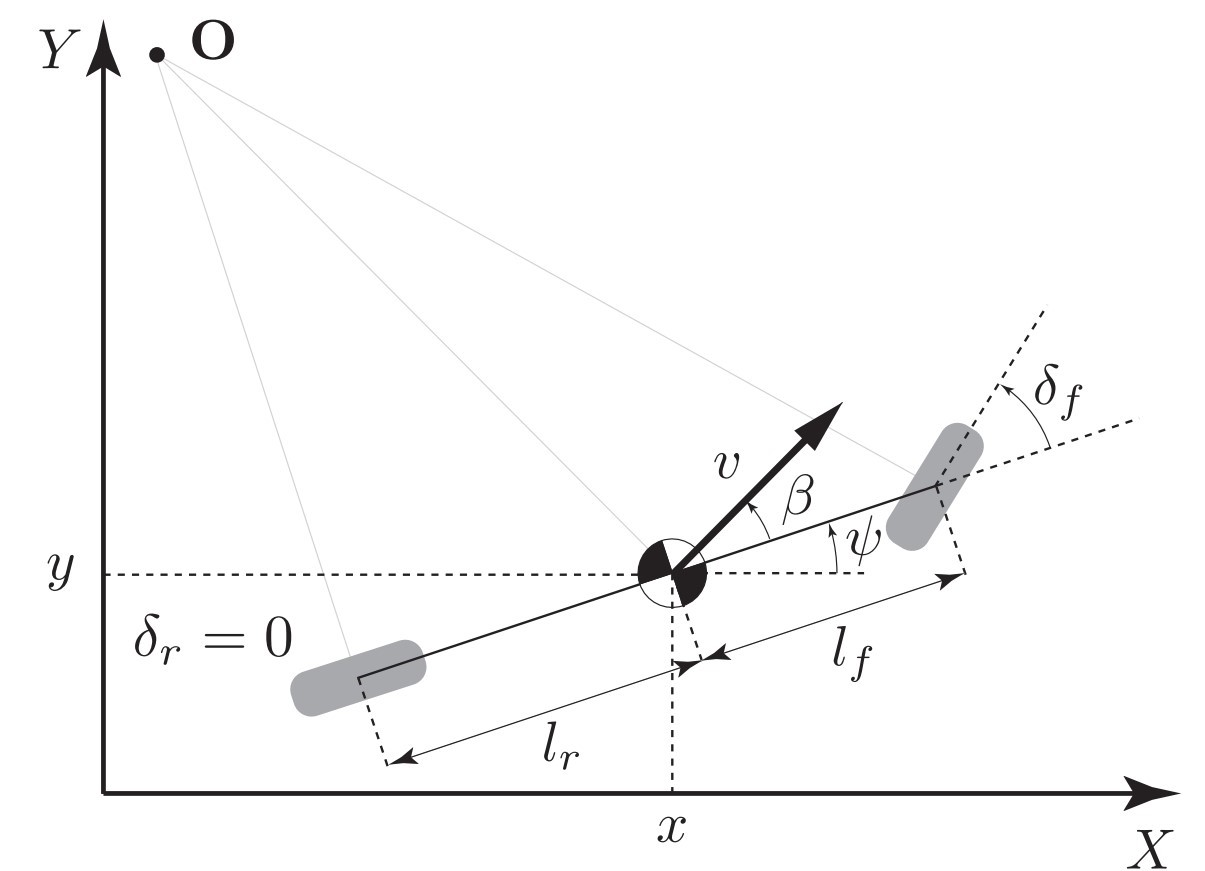
\includegraphics[width=0.5\textwidth]{Figures/Bicycle_model.jpg}
    \caption{Bicycle kinematic vehicle model}
    \label{fig:Bicycle_kin}
\end{figure}
This model can be further simplified assuming that, as in the most of commercial vehicles, only the front wheels are able to steer, so the rear steering angle $\delta_r$ is constant and equal to 0.\\
Standard MPC controller works on linear systems, so we decided to implement a linearized version of the Bicycle Model to feed the controller. This linearized model is described by the following State Space equations:
\begin{equation}
    \label{equation:dynamic1}
    \Dot{x} = Ax + Bu 
\end{equation}
\begin{equation}
    \label{equation:dynamic2}
    y = Cx + Du 
\end{equation}
with:

\begin{equation}
\label{equation:sys_bicycle_kin}
   \begin{aligned}
    x = 
        \begin{bmatrix} % STATES
        X \\ 
        Y \\
        \psi \\
        v \\
        \end{bmatrix}\quad
    A =
        \begin{bmatrix} % MATRIX A
       0 & 0 & -Vsin(\psi) & cos(\psi)\\ 
       0 & 0 & Vcos(\psi) & sin(\psi) \\
       0 & 0 & 0 & \frac{tan(\delta)}{l_r + l_f}\\
       0 & 0 & 0 & 0 \\
        \end{bmatrix}\quad
    B = 
        \begin{bmatrix} % MATRIX B
        0 & 0\\ 
        0 & 0 \\
        0 & \frac{Vtan(\delta)^2 + 1}{l_r + l_f}\\
        1 & 0 \\
        \end{bmatrix}\\[10pt]
    u =
        \begin{bmatrix} % INPUTS
        Throttle \\
        \delta \\
        \end{bmatrix}\quad\quad\quad
    C = I^{4\times 4}\quad\quad\quad\quad\quad
    D =
        \begin{bmatrix} % MATRIX A
      0 & 0 & 0 & 0\\
      0 & 0 & 0 & 0\\
        \end{bmatrix}
    \end{aligned}
\end{equation} 

These matrices are obtained evaluating the Taylor expansion of the non linear bicycle model, as explained in the MathWorks example \cite{StaticObs}.\\
A more complex vehicle model can be useful to test the performance of the controller to be developed. The \textit{Dynamic Bicycle Model} \cite{7225830} can be built starting from the previous non linear model, deriving the following second order derivative equations:
\begin{align}
    \ddot{x} = \dot{\psi}\dot{y} + Throttle\\
    \ddot{y} = -\dot{\psi}\dot{x} + \frac{2}{m}\left(F_fcos(\delta) + F_r\right)\\
    \ddot{\psi} = \frac{2}{I_z}\left(l_fF_f - l_rF_r\right)\\
    \dot{X} = \dot{x}cos(\psi) - \dot{y}sin(\psi)\\
    \dot{Y} = \dot{x}sin(\psi) + \dot{y}cos(\psi)\\
\end{align}
where $m$ is the mass of the vehicle, $I_z$ is the inertia of the vehicle with respect to the vertical axle passing for the CoG of it, while $F_f$ and $F_r$ are respectively the side slip forces acting on the front and rear wheels, and they can be evaluated as:
\begin{align}
    F_f = 2C_f\left(\delta - \theta_f\right)\\
    F_r = 2C_r\left(-\theta_r\right)
\end{align}
with $C_i$ side slip friction coefficient of the i-th wheel couple and $\theta_i$ side slip angle of the wheels.\\
Tyre side slip angles can be approximated by the following equations:
\begin{equation}
    \theta_f=tan^{-1}\left(\frac{\dot{y} + l_f\dot{\psi}}{\dot{x}}\right)
\end{equation}
\begin{equation}
    \theta_r=tan^{-1}\left(\frac{\dot{y} - l_r\dot{\psi}}{\dot{x}}\right)
\end{equation}
The models introduced are, more or less, independent of the longitudinal dynamics of the vehicle, since they link this dynamic with a simple coefficient, that is the $Throttle$. In our model, this coefficient should be considered as an acceleration of the vehicle, and it can be both positive (driving) or negative (braking). Range of values for this parameter is dependent on lots of variables, of course, such as the engine power, the vehicle mass and inertia, the ground type, the rubber of the wheels and so on. Our assumption is to give a fixed interval for this parameter, to simulate a small commercial vehicle on dry asphalt, which can have a maximum acceleration of $4 m/s^2$ and a maximum braking deceleration of $-0.8g$. To summarize:
\begin{itemize}
    \item $Throttle \in [-7.85, 4.00]m/s^2$
    \label{item:Throttle}
\end{itemize}
Parameters considered for the bicycle model are taken from real vehicle data \cite{10.2307/44733900} and are reported in the following table:

\begin{table}[H]
\resizebox{\textwidth}{!}{%
\begin{tabular}{|l|l|r|r|r|r|r|}
\hline
\textbf{ID} &
  \textbf{Vehicle name} &
  \multicolumn{1}{l|}{\textbf{Wheel base {[}$m${]}}} &
  \multicolumn{1}{l|}{\textbf{l\_r {[}$m${]}}} &
  \multicolumn{1}{l|}{\textbf{l\_f {[}$m${]}}} &
  \multicolumn{1}{l|}{\textbf{Mass {[}$kg${]}}} &
  \multicolumn{1}{l|}{\textbf{Inertia {[}$kg \cdot m^2${]}}} \\ \hline
1 & \textit{Hyundai Azera }    & 2.843 & 1.738 & 1.105 & 1200 & 1000 \\ \hline
2 & \textit{BMW 325i}          & 2.570 & 1.369 & 1.201 & 1251 & 2027 \\ \hline
3 & \textit{Ford E150 }        & 3.505 & 1.634 & 1.871 & 2995 & 6536 \\ \hline
4 & \textit{Suzuki Samurai}    & 2.032 & 0.870 & 1.162 & 1229 & 1341 \\ \hline
5 & \textit{Volkswagen Beetle} & 2.408 & 0.996 & 1.412 & 857  & 1289 \\ \hline
\end{tabular}%
}
\caption{Vehicle data considered for development and validation}
\label{tab:vehicle_data}
\end{table}
Values reported in the table \ref{tab:vehicle_data} are stored in a MATLAB file and can be accessed through the \textit{loadParameters} function, which take as input the vehicle ID and returns the parameters associated with that vehicle. To avoid to call improperly this function, a default parameters set as been provided with the following values:
\begin{table}[H]
\resizebox{\textwidth}{!}{
\begin{tabular}{|l|r|r|r|r|r|}
\hline
\textbf{Vehicle name} &
  \multicolumn{1}{l|}{\textbf{Wheel base {[}$m${]}}} &
  \multicolumn{1}{l|}{\textbf{l\_r {[}$m${]}}} &
  \multicolumn{1}{l|}{\textbf{l\_f {[}$m${]}}} &
  \multicolumn{1}{l|}{\textbf{Mass {[}$kg${]}}} &
  \multicolumn{1}{l|}{\textbf{Inertia {[}$kg \cdot m^2${]}}} \\ \hline
\textit{Default}    & 2 & 1 & 1 & 1000 & 1000 \\ \hline
\end{tabular}
}
\end{table}
We used data of vehicle 1, \textit{Hyundai Azera}, for the development phase, where mass and inertia are not the real ones of the vehicle, but are given with realistic values, while other data of the previous table \ref{tab:vehicle_data} are meant to be used in the validation phase, to test the controller with different vehicles.
For what concern the side slip friction values, we considered two fixed values for all the vehicles that are:
\begin{itemize}
    \item $C_f$ $=$ $1.0745\times10^5$ N/rad
    \item $C_r$ $=$ $1.9032\times10^5$ N/rad
\end{itemize}
while in the \textit{"default"} condition they are both $10^5$ N/rad.

\subsection{Model comparison}
As specified in the subsection \ref{partitioning_subsection} we have decided to use two models, a simplified and linearized model for the MPC and a more complex one for the simulation of the model. The former is defined as \textit{Kinematic Bicycle Model} and the latter as \textit{Dynamic Bicycle Model}.
Hence we have decided to test both of these systems to show how they behave with different throttle and steering inputs using the \textit{Simulink Test} tool. Thus, the tests performed are:
\begin{itemize}
    \item \textbf{Free evolution test}: this test has been performed considering a constant steering of $0^{\circ}$ and a constant throttle of 0 $m/s^2$;
    \item \textbf{Only throttle test}: this test has been performed keeping the steering angle constant and equal to $0^{\circ}$ and varying the throttle as shown in Figure \ref{fig:InputThrottle};
    \item \textbf{Constant steering test}: this test has been performed keeping the throttle constant and equal to 0 $m/s^2$ and the steering angle constant and equal to $2^{\circ}$;
    \item \textbf{Ramp steering test}: this test has been performed keeping the throttle equal to 0 $m/s^2$ and giving a ramp steering angle signal (varying linearly from $0^{\circ}$ to $36^{\circ}$);
    \item \textbf{Small sinusoidal steering test}: this test has been performed keeping the throttle constant and equal to 0 $m/s^2$ and giving a sinusoidal steering angle signal with frequency 0.2 $Hz$ and amplitude $5^{\circ}$;
    \item \textbf{Big sinusoidal steering test}: here we have performed the same test as before (sinusoidal steering input) but with a larger amplitude of the sine wave ($15^{\circ}$);
    \item \textbf{Combined test 1}: this test has been performed keeping the steering angle constant and equal $2^{\circ}$ and varying the throttle as shown in Figure \ref{fig:InputThrottle};
    \item \textbf{Combined test 2}: this test has been performed keeping the throttle equal to 0.2 $m/s^2$ and giving a ramp steering angle signal (varying linearly from $0^{\circ}$ to $36^{\circ}$).
\end{itemize}

\begin{figure}[H]
    \centering
    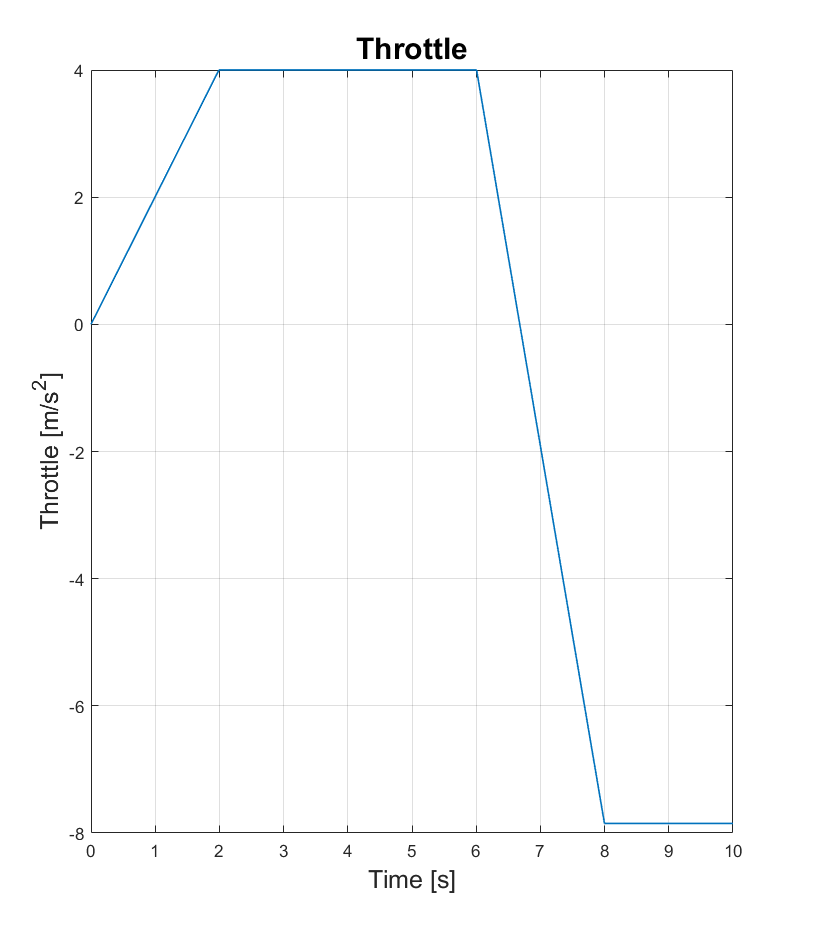
\includegraphics[width=0.65\textwidth]{Figures/InputThrottle.png}
    \caption{Throttle Input used in \textit{Only throttle test} and \textit{Combined test 1}. Maximum and minimum values are coherent with the range described in Section \ref{item:Throttle} in order to explore the whole set of throttle values.}
      \label{fig:InputThrottle}
\end{figure}






\subsubsection{Simulink Test}
The above-mentioned tests have been performed using the \textit{Simulink Test} tool implemented by MathWorks. Simulink Test provides tools for authoring, managing, and executing systematic, simulation-based tests of models, generated code, and simulated or physical hardware. It includes simulation, baseline, and equivalence test templates that let you perform functional, unit, regression, and back-to-back testing using software-in-the-loop (SIL), processor-in-the-loop (PIL), and real-time hardware-in-the-loop (HIL) modes. With Simulink Test you can create non-intrusive test harnesses to isolate the component under test. You can define requirements-based assessments using a text-based language, and specify test input, expected outputs, and tolerances in a variety of formats. \cite{SimulinkTest}

\subsubsection{Results analysis}

Exploiting Simulink Test, we have created two test harnesses : \textit{Dynamic} and \textit{Kinematic}. Those are referred to the models described at the beginning of this section. Then, we have executed an Equivalence Test which allowed us to make a comparison between two simulations. In particular, the Dynamic Model has been considered as the \textit{baseline} which our Kinematic Model has been compared to in the test. The baseline represents the expected output being more accurate than the Kinematic model, which in turn is called \textit{Compare to} model inside the Simulink Test automatic report generator\footnote{The ``Model Comparison - Test Report" file generated by Simulink Test is included in the /Documentation/Test Reports/ file path}. 
Since these tests aim to give a qualitative analysis of the two models and compare them, we have not included equivalence criteria.
The only parameter we have set up is the relative tolerance assigning to it a value of 1\% in order to ignore the negligible offsets between the dynamic model and the kinematic model.\\
Figure \ref{fig:trajectories} shows the results of the simulations we have carried out. 
As shown in Figures \ref{subfig:free_evo} and \ref{subfig:only_throttle} respectively, as expected the two models behave in the same way when no inputs are present or when only the longitudinal input (throttle) is changed. \\ Another relevant result is shown in Figures \ref{subfig:small_sinusoidal} and \ref{subfig:big_sinusoidal}: as long as the amplitude of the sinusoidal input is fairly small, the two models behave in a similar fashion but the greater the amplitude of the sinusoidal input, the greater the deviation of the kinematic model from the dynamic one.\\
The other images shown below, underline as well the offset between the two vehicle models, which is due to the fact that when using the dynamic model we take into account lateral slips which are not considered in the kinematic model.


\begin{figure}[H]
\centering

    \begin{subfigure}{.5\textwidth}
    \centering
   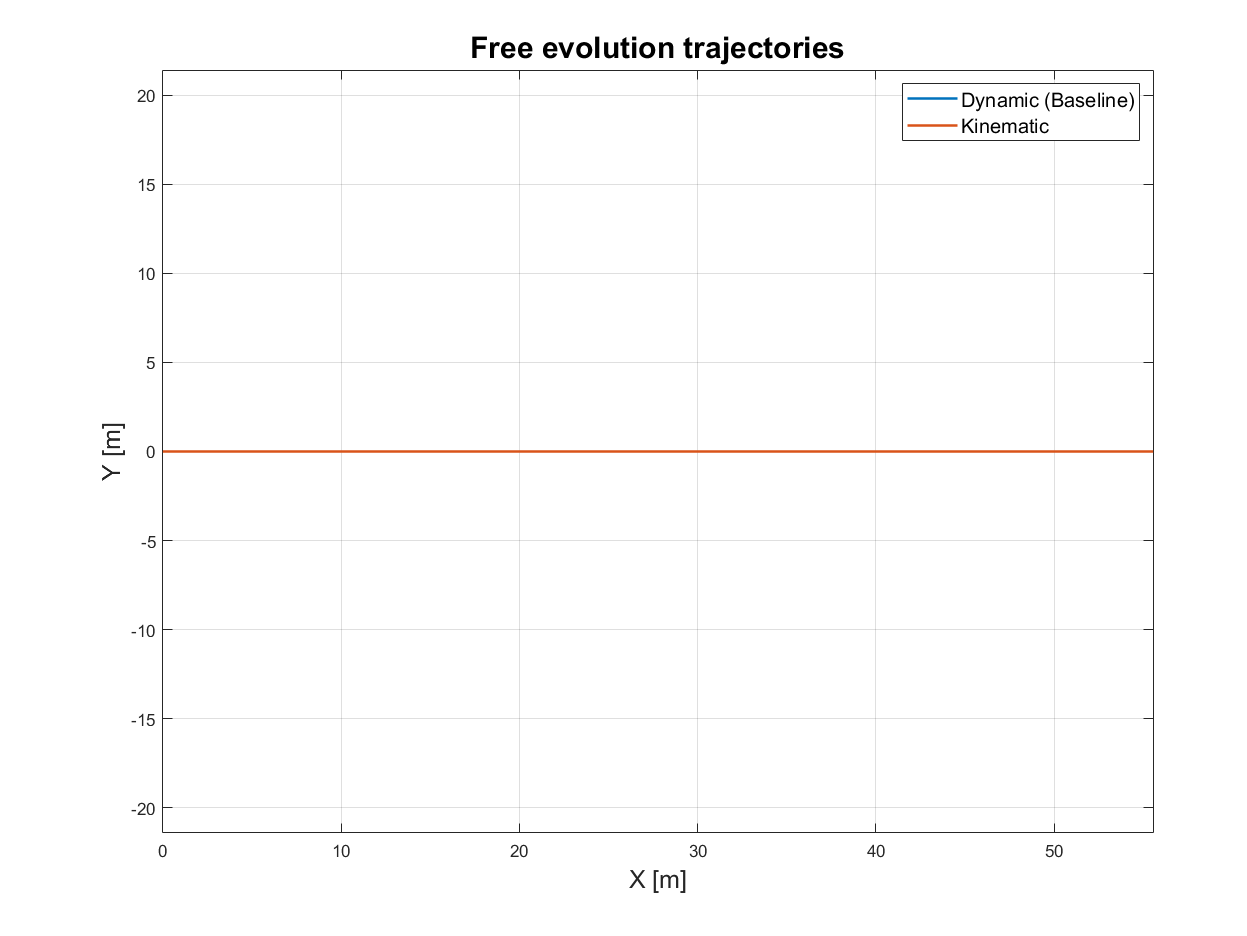
\includegraphics[width=0.8\textwidth,keepaspectratio]{Figures/Free_evo_traj.png}
    \caption{Free evolution test - trajectories}
    \label{subfig:free_evo}
    \end{subfigure}%
    \begin{subfigure}{.5\textwidth}
    \centering
    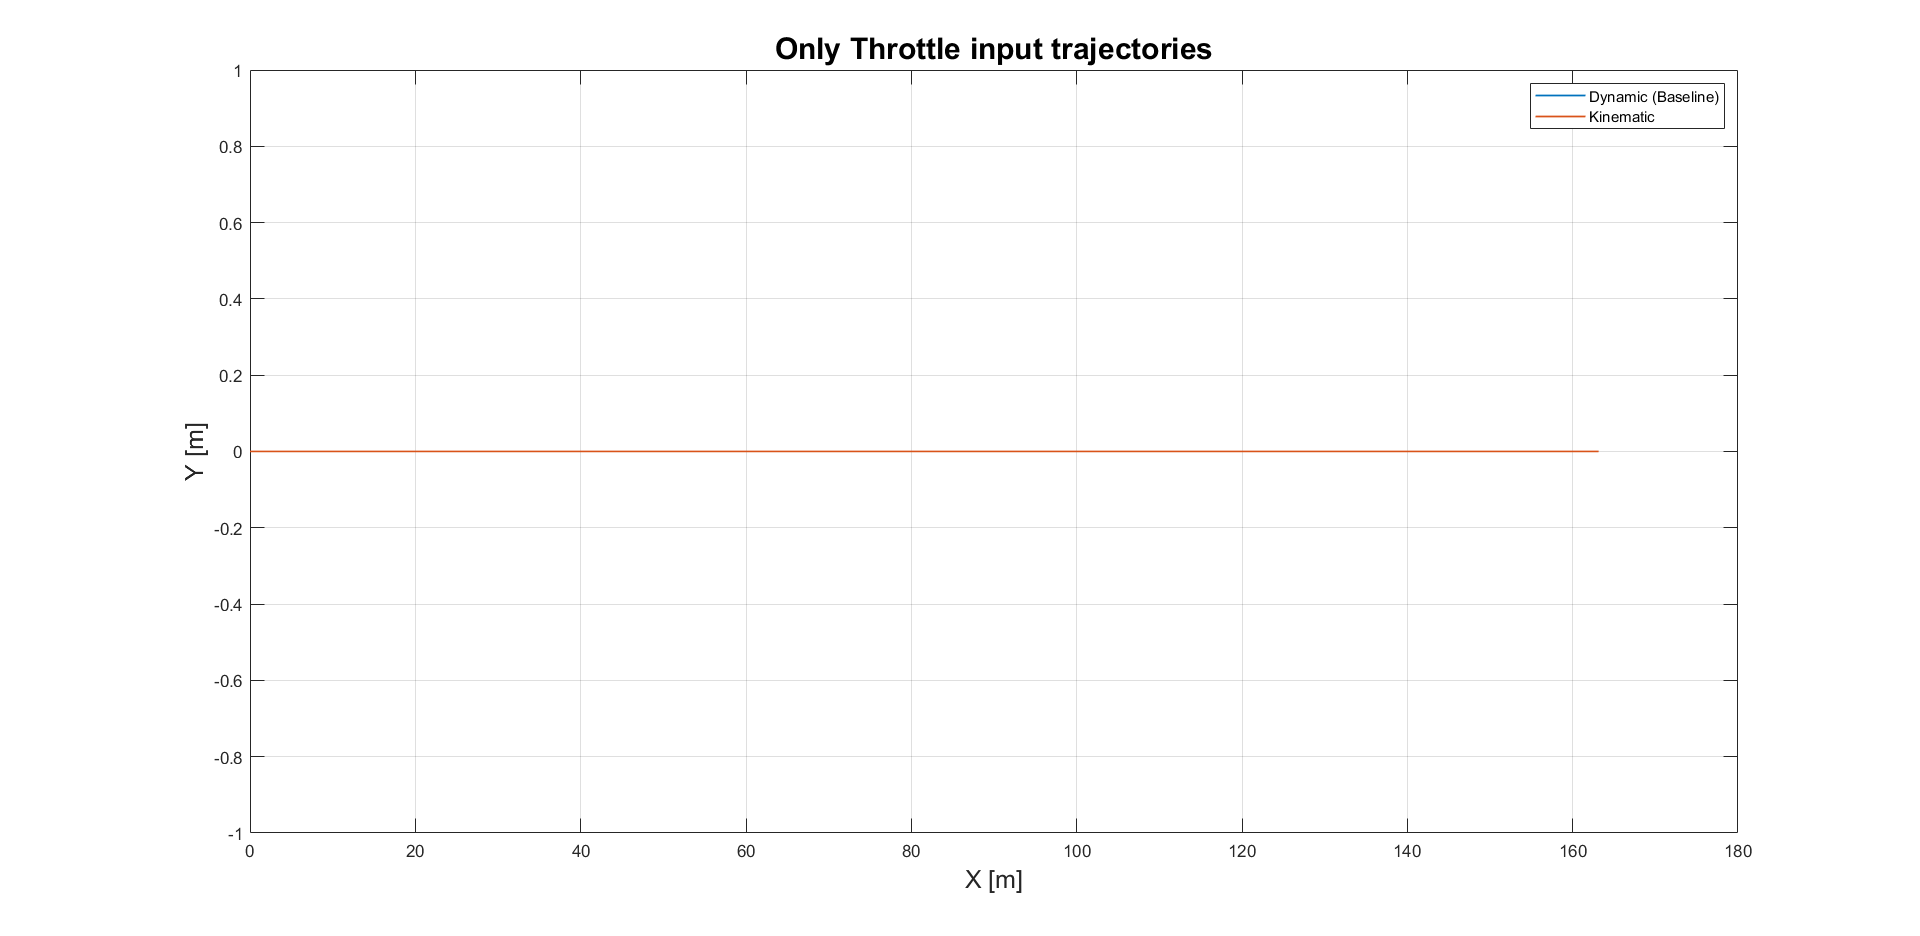
\includegraphics[width=0.8\textwidth,keepaspectratio]{Figures/Throttle_traj.png}
    \caption{Only throttle test - trajectories}
    \label{subfig:only_throttle}
    \end{subfigure}
    
    \vspace{10mm}
    
    \begin{subfigure}{.5\textwidth}
    \centering
   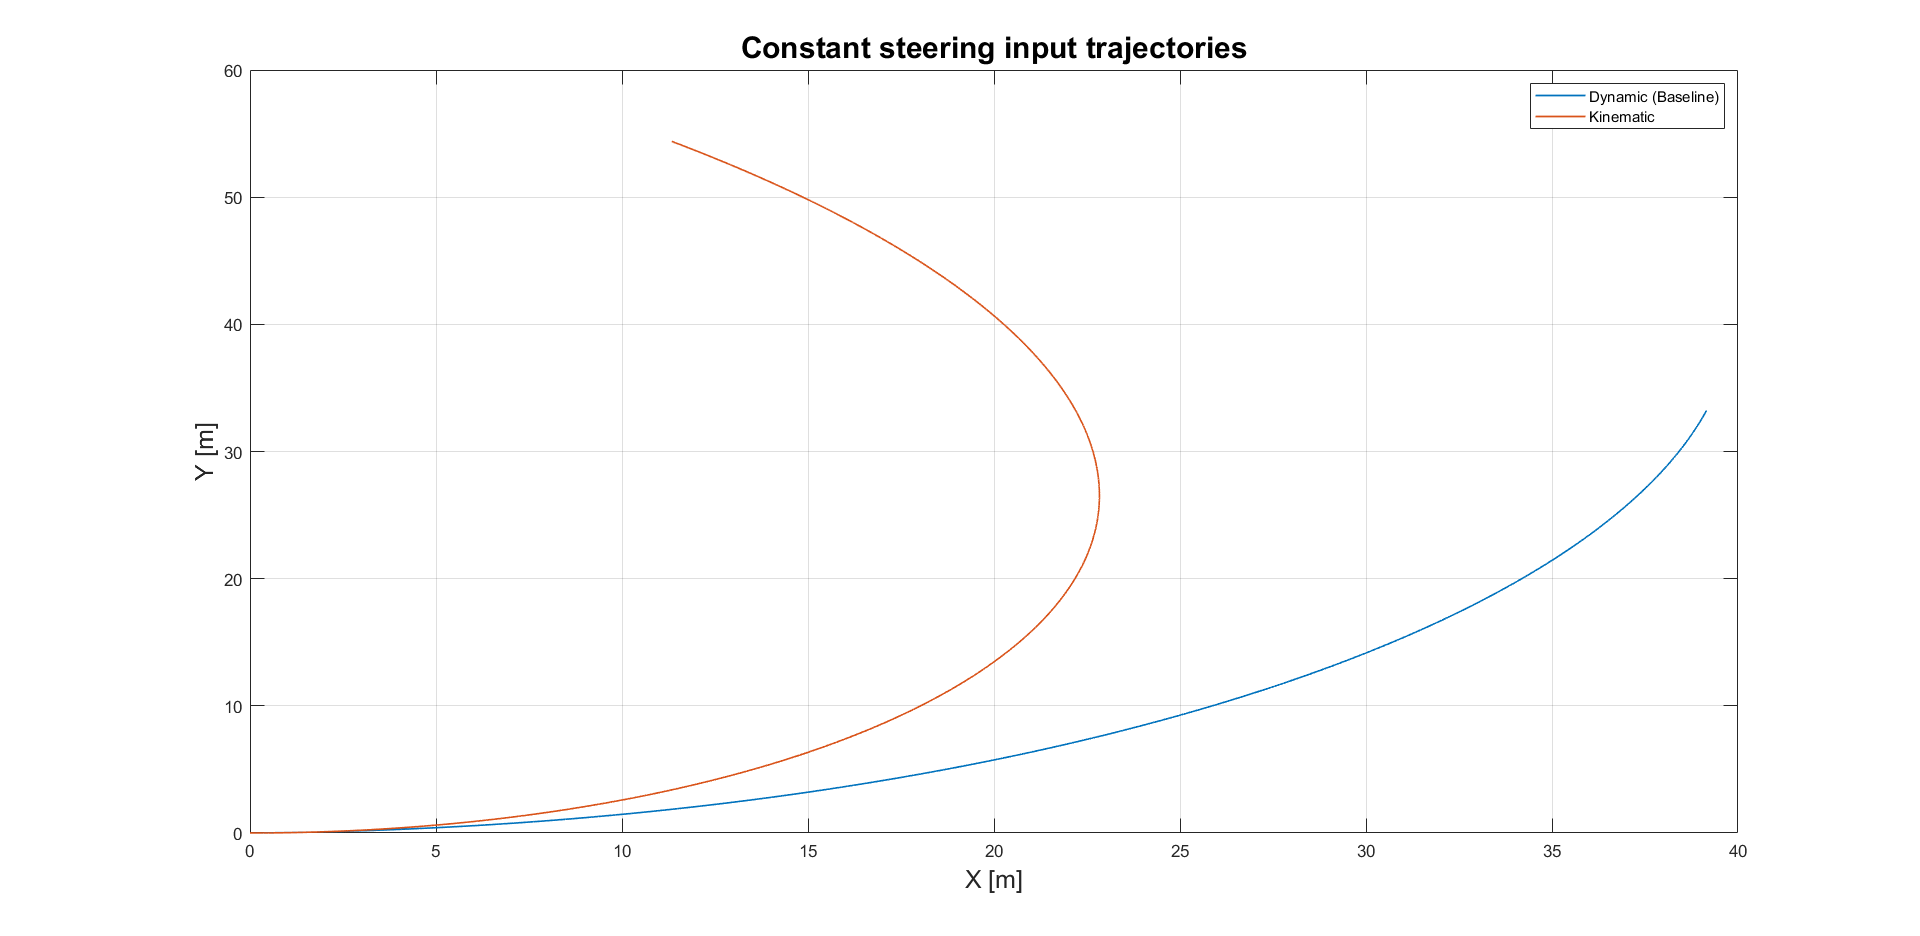
\includegraphics[width=0.8\textwidth,keepaspectratio]{Figures/Const_steer_traj.png}
   \caption{Constant steering test - trajectories}
   \label{subfig:const_steer}
    \end{subfigure}%
    \begin{subfigure}{.5\textwidth}
    \centering
    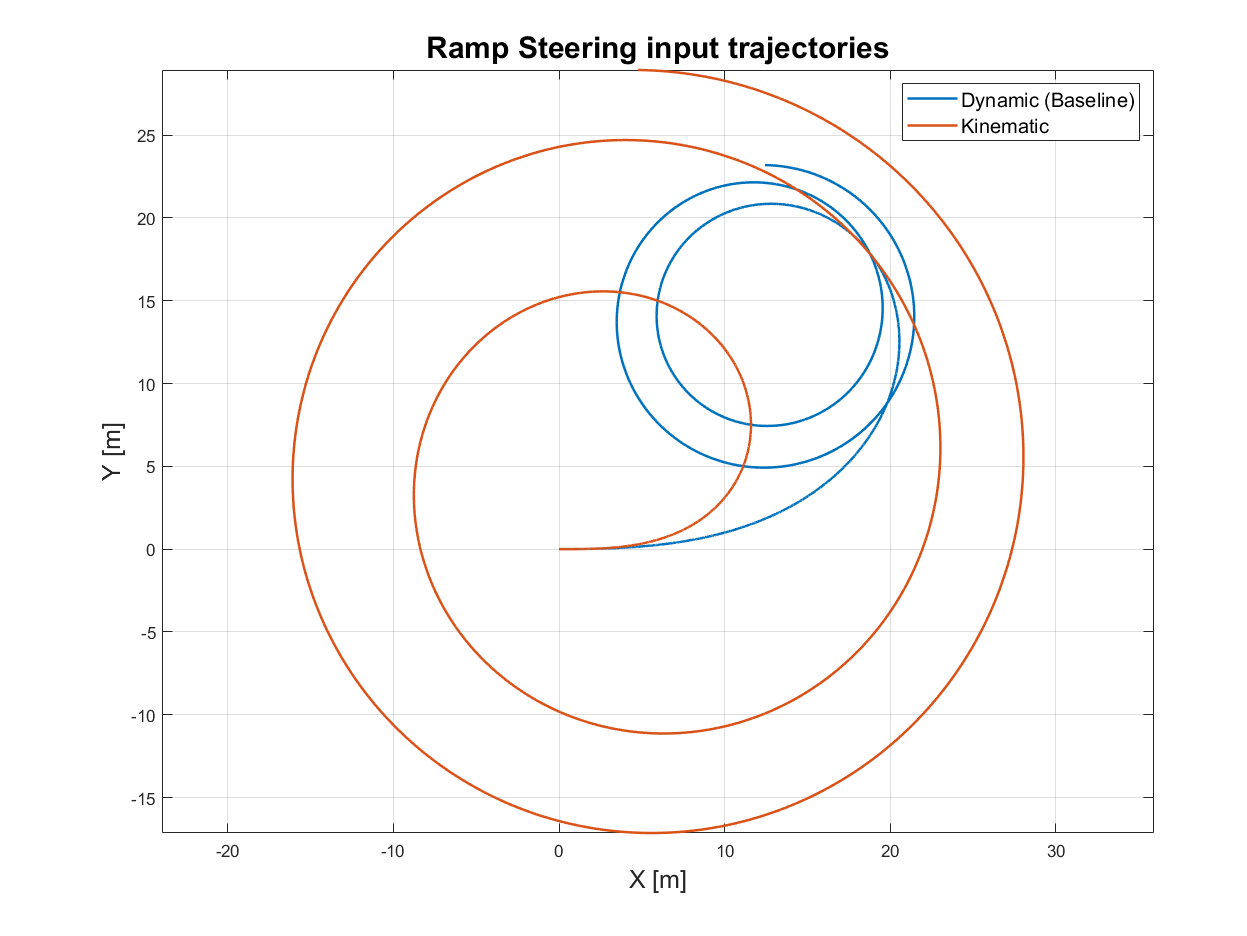
\includegraphics[width=0.8\textwidth,keepaspectratio]{Figures/Ramp_traj.png}
    \caption{Ramp steering test - trajectories}
    \label{subfig:ramp_steer}
    \end{subfigure}
    
     \vspace{10mm}
     
    \begin{subfigure}{.5\textwidth}
    \centering
   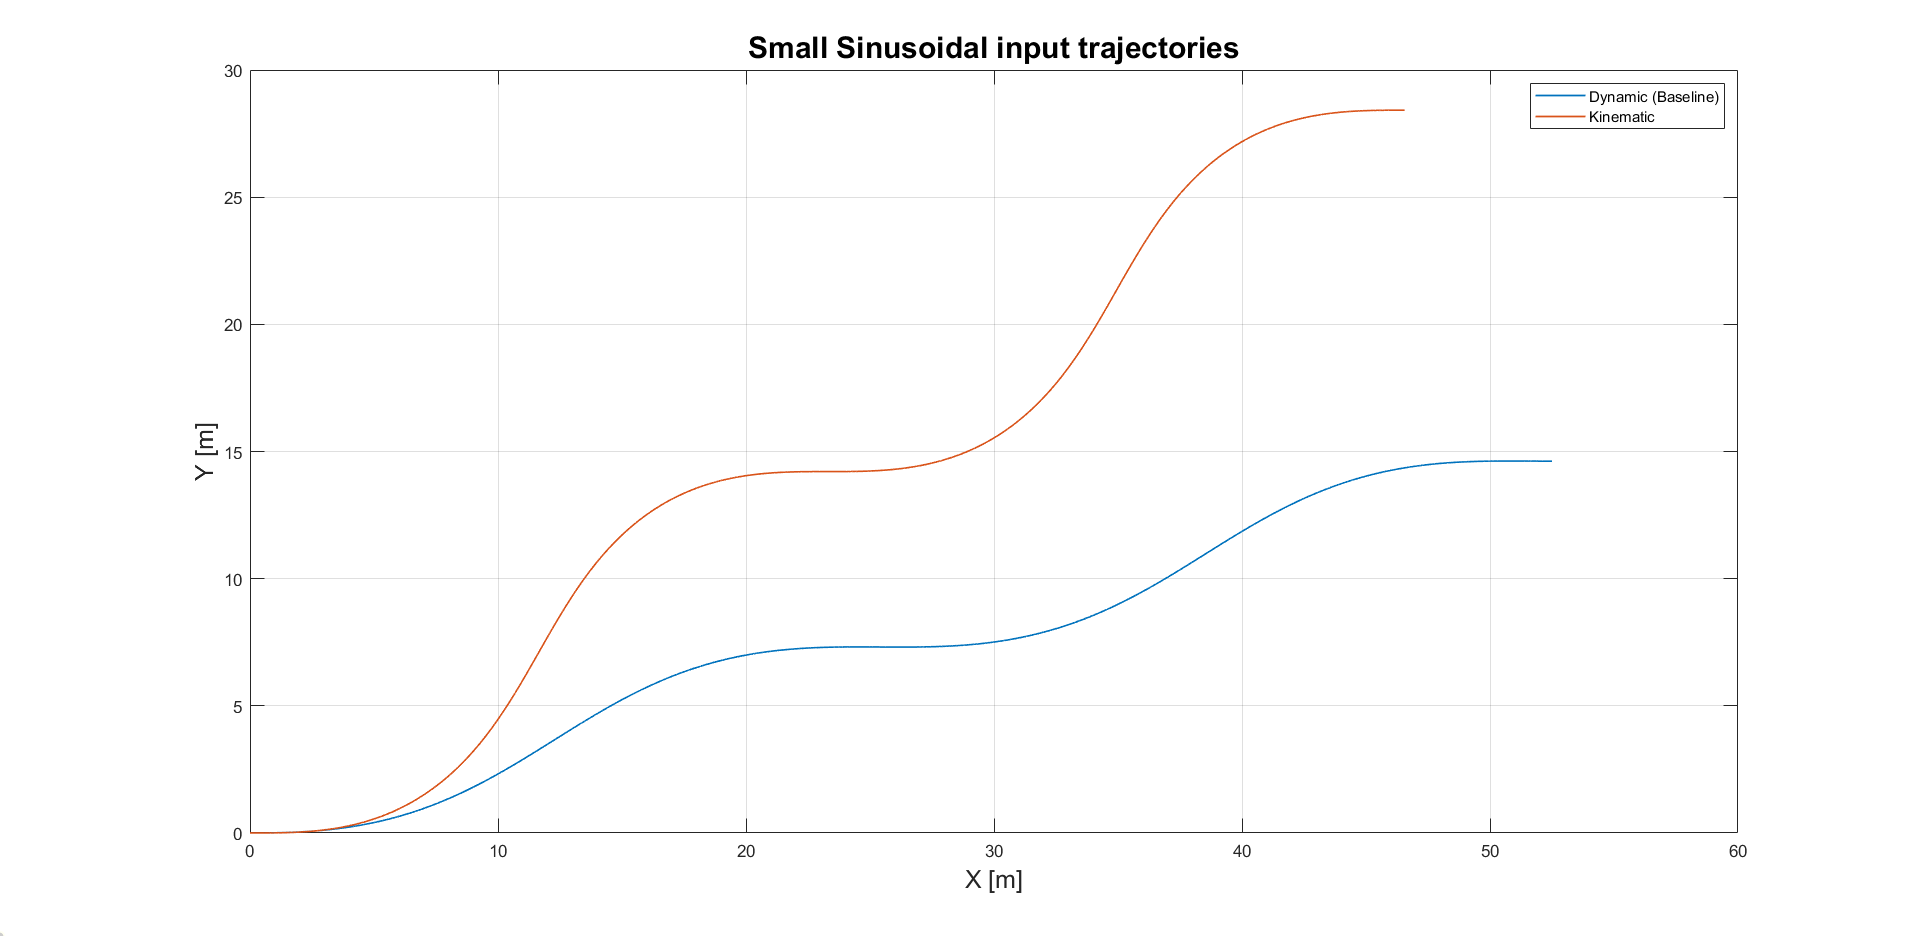
\includegraphics[width=0.8\textwidth,keepaspectratio]{Figures/Small_sin_traj.png}
   \caption{Small sinusoidal test - trajectories}
   \label{subfig:small_sinusoidal}
    \end{subfigure}%
    \begin{subfigure}{.5\textwidth}
    \centering
    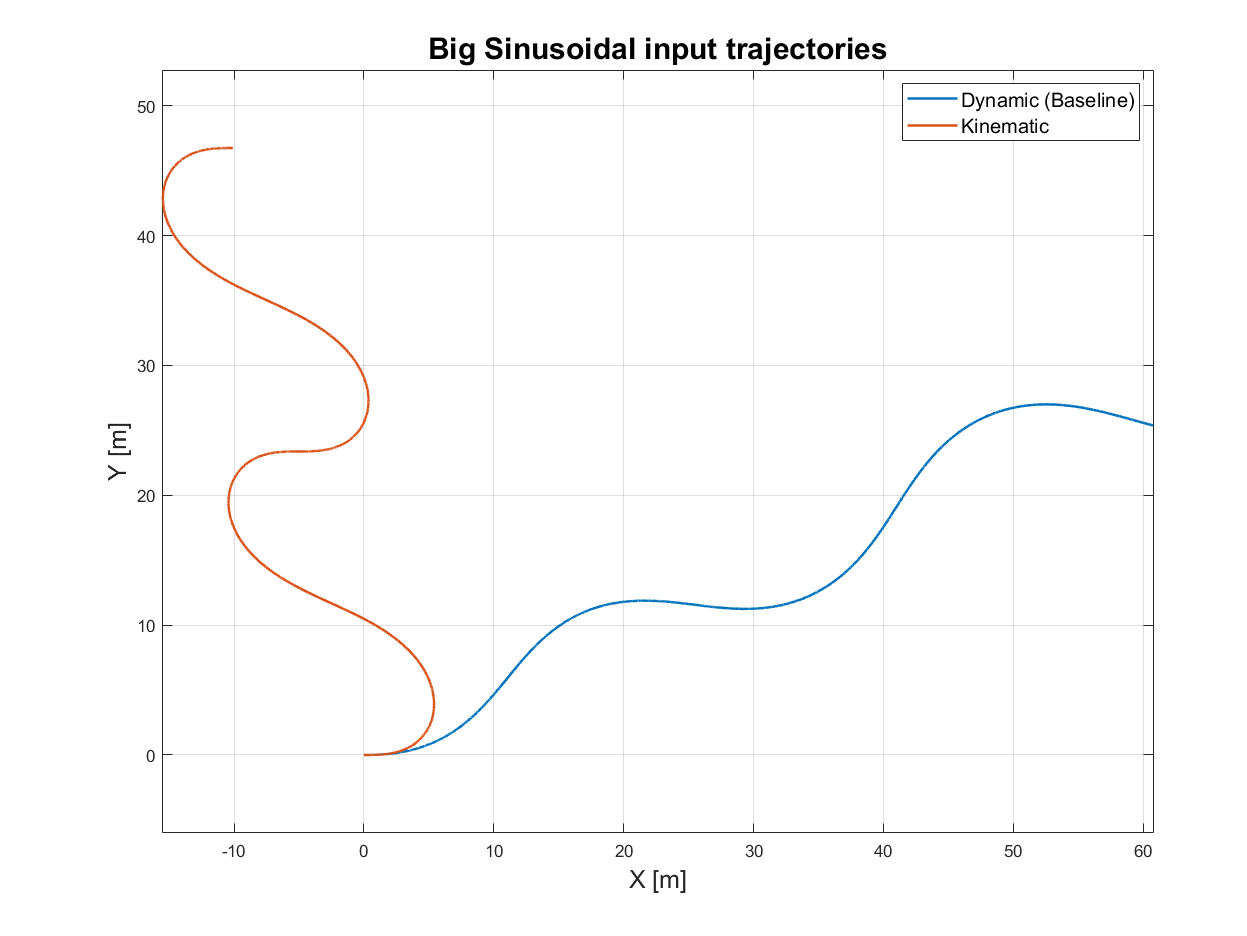
\includegraphics[width=0.8\textwidth,keepaspectratio]{Figures/Big_sin_traj.png}
    \caption{Big sinusoidal test - trajectories}
    \label{subfig:big_sinusoidal}
    \end{subfigure}
    
     \vspace{10mm}
    
    \begin{subfigure}{.5\textwidth}
    \centering
  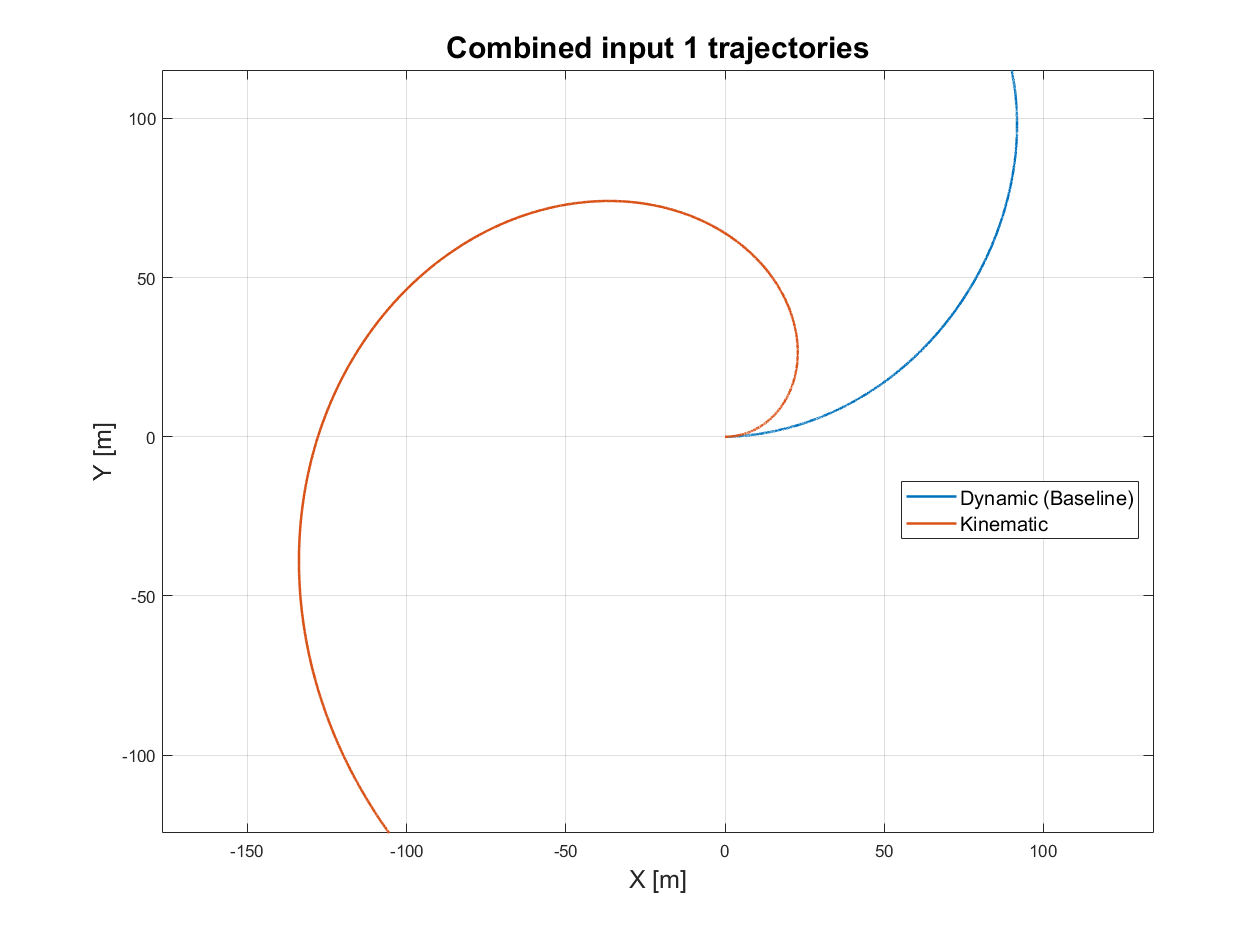
\includegraphics[width=0.8\textwidth,keepaspectratio]{Figures/Comb1_traj.png}
    \caption{Combined 1 test - trajectories}
    \label{subfig:Comb_1}
    \end{subfigure}%
    \begin{subfigure}{.5\textwidth}
    \centering
  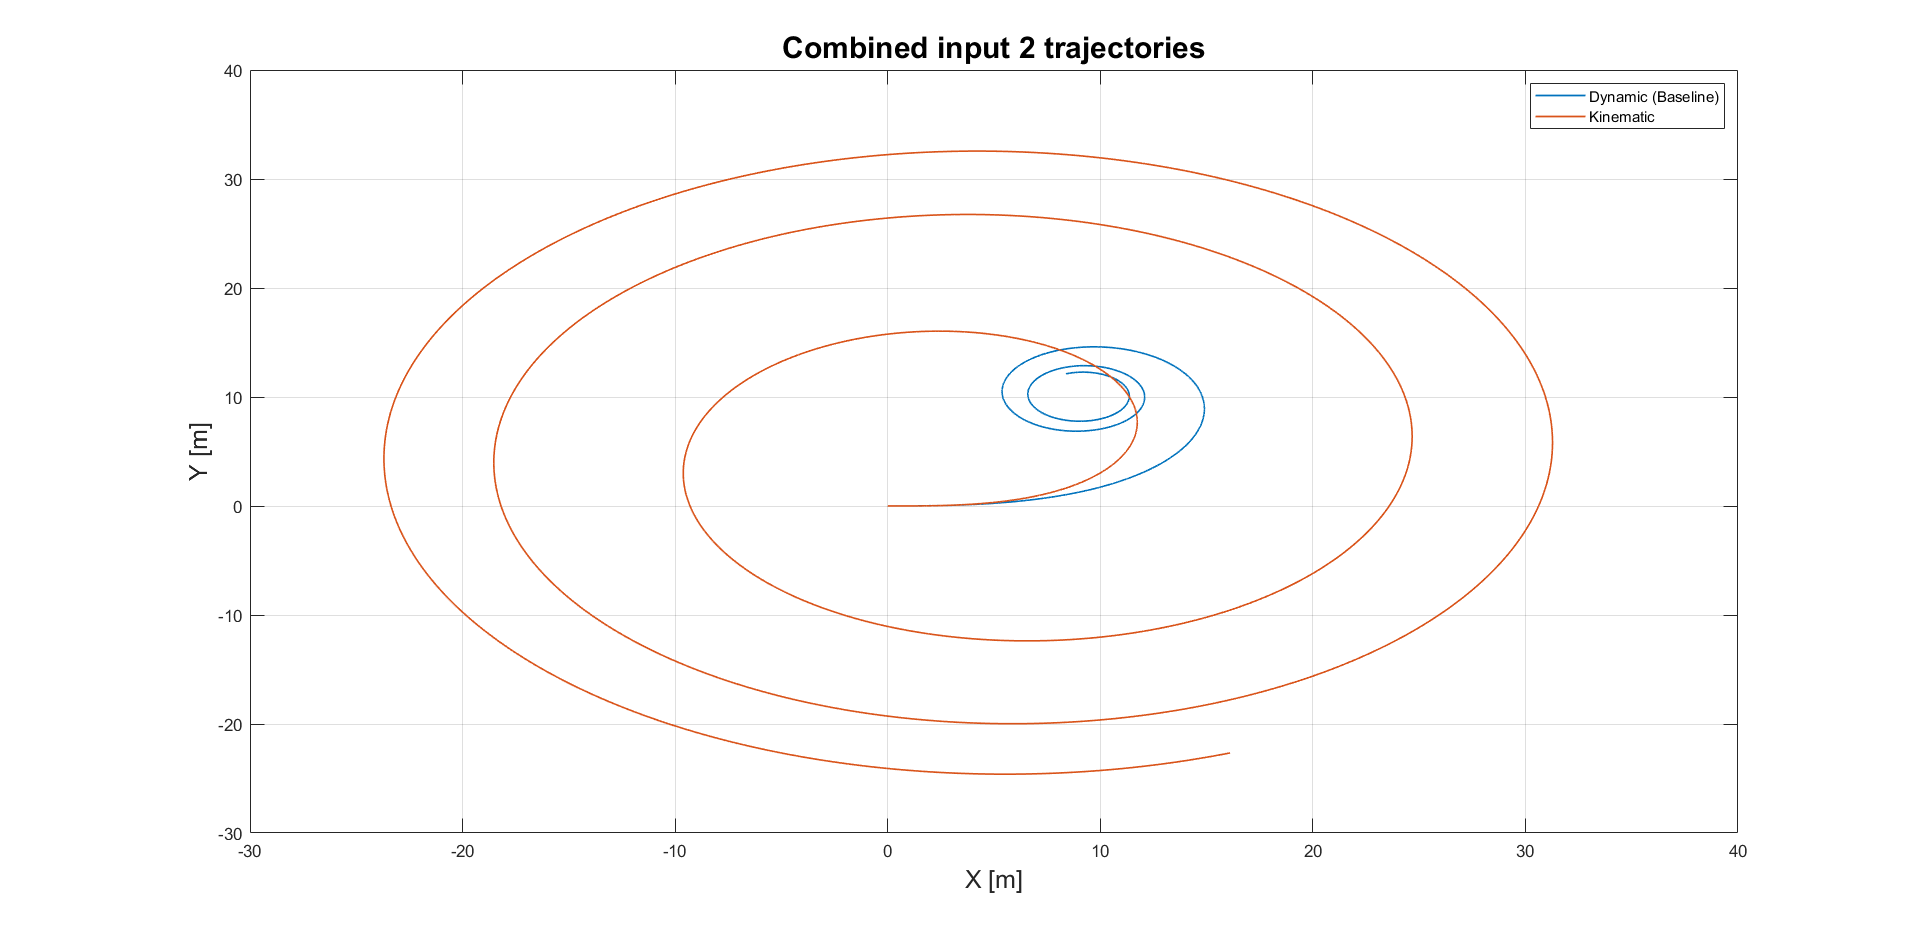
\includegraphics[width=0.8\textwidth,keepaspectratio]{Figures/Comb2_traj.png}
    \caption{Combined 2 test - trajectories}
    \label{subfig:Comb_2}
    \end{subfigure}
    
    \caption{Output trajectories of the test set}
    \label{fig:trajectories}
\end{figure}
\pagebreak


After the analysis of the results, we decided to provide to the MPC the linearized bicycle model for the vehicle plant, because the controller is usually updated with the current state in some fractions of a second, and for this reason the differences between the model and the \textit{``Real World"} system, that in our case is represented by the dynamic model, shouldn't affect too much the behaviour of the controller itself. As a matter of fact, by looking at the images above it is clear that the difference between the two models output is negligible at the first time steps of the simulation.\\
Moreover, as already discussed in this section, the performances of the two models are very similar if compared with small inputs, and this condition is fulfilled if we consider to use our controller in normal driving scenarios, such as, for instance, an highway.\\
Keeping in mind these assumptions, we go on with the project, considering to apply a change in the vehicle model for the MPC if we are not able to achieve good results with this one.